% 1981 年全国卷（理科）第 10 题：以 AB 为直径的半圆及其内接正方形 CDEF（按源卷布局）。
% 圆心 O 为原点、半径 sqrt(5)/2；F、C 关于 O 对称，边长为 1，E、D 在半圆上。
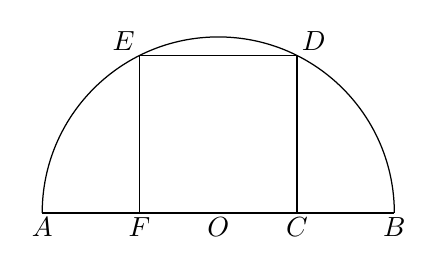
\begin{tikzpicture}[scale=2.0, line width=0.45pt,
  every node/.style={inner sep=1.5pt}]
  \pgfmathsetmacro{\R}{sqrt(5)/2}
  \coordinate (O) at (0,0);
  \coordinate (A) at (-\R,0);
  \coordinate (B) at (\R,0);
  \coordinate (F) at (-0.5,0);
  \coordinate (C) at (0.5,0);
  \coordinate (E) at (-0.5,1);
  \coordinate (D) at (0.5,1);
  % 半圆与直径 AB
  \draw (A) arc (180:0:\R);
  \draw (A) -- (B);
  % 内接正方形 CDEF
  \draw (F) -- (E) -- (D) -- (C) -- cycle;
  \node[anchor=north] at (A) {$A$};
  \node[anchor=north] at (F) {$F$};
  \node[anchor=north] at (O) {$O$};
  \node[anchor=north] at (C) {$C$};
  \node[anchor=north] at (B) {$B$};
  \node[anchor=south east] at (E) {$E$};
  \node[anchor=south west] at (D) {$D$};
\end{tikzpicture}
